% Ссылка в тексте: (приложение~Л)
\chapter{СКРИНШОТЫ MVP И E2E-ДОКАЗАТЕЛЬСТВО РАБОТЫ AI-МЕТОДИСТА}

В~приложении приведены скриншоты, полученные из~локального
end-to-end-сценария платформы Adapstory School. Тестовый сценарий
имитирует загрузку исходного материала, запуск AI-методиста,
отображение состояния пайплайна, проверку качества, источники,
provenance блоков курса и~метрики дипломной валидации.

Скриншоты сформированы локальным Playwright end-to-end-прогоном.
Для воспроизводимости вместе с~изображениями сохранены JSON-ответы:
\texttt{figures/ui/ai-methodist-status-result.json} и
\texttt{figures/ui/ai-methodist-provenance-result.json}.

\section*{Л.1 --- Загрузка исходных материалов}

На~рисунке~\ref{fig:ai-methodist-upload} показан первый шаг сценария:
пользователь добавляет документ или~краткое описание курса. Этот экран
подтверждает, что MVP поддерживает работу от~источников, а~не~только
генерацию по~свободному промпту.

\begin{figure}[p]
  \centering
  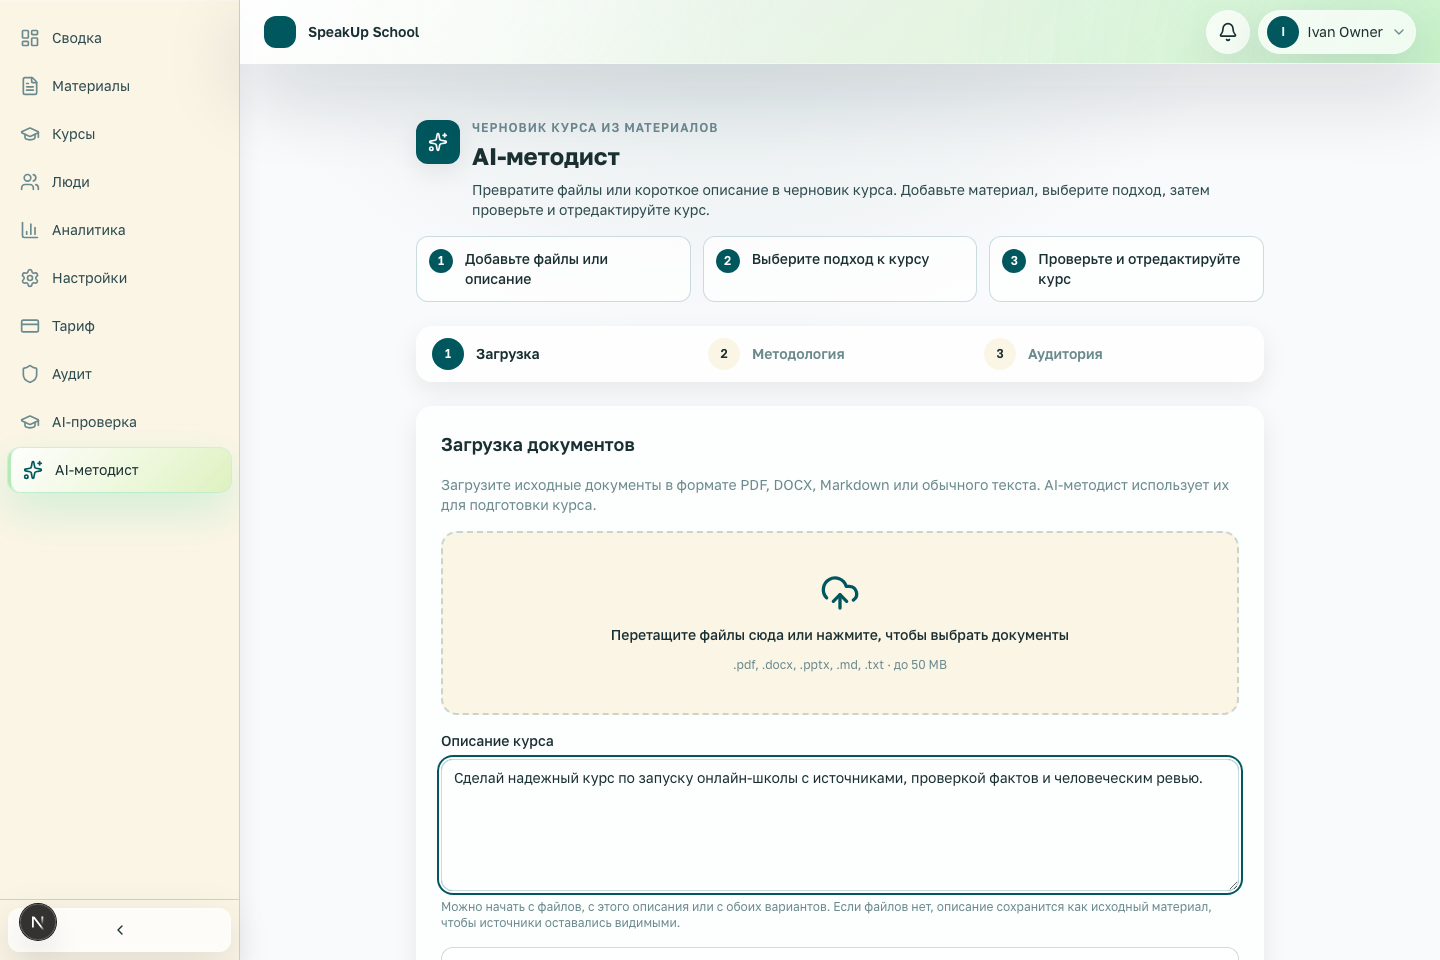
\includegraphics[width=0.98\textwidth]{figures/ui/ai-methodist-01-upload.png}
  \caption{Экран загрузки источников и описания курса для AI-методиста}
  \label{fig:ai-methodist-upload}
\end{figure}

\section*{Л.2 --- Статус пайплайна генерации}

После запуска платформа открывает экран состояния пайплайна
(рисунок~\ref{fig:ai-methodist-status}). На~нём видны этапы анализа
источников, построения структуры, генерации контента, проверки фактов,
ревью и~верификации. В~той~же рабочей области отображаются модель,
токены, оценочная стоимость и~оценка качества.

\begin{figure}[p]
  \centering
  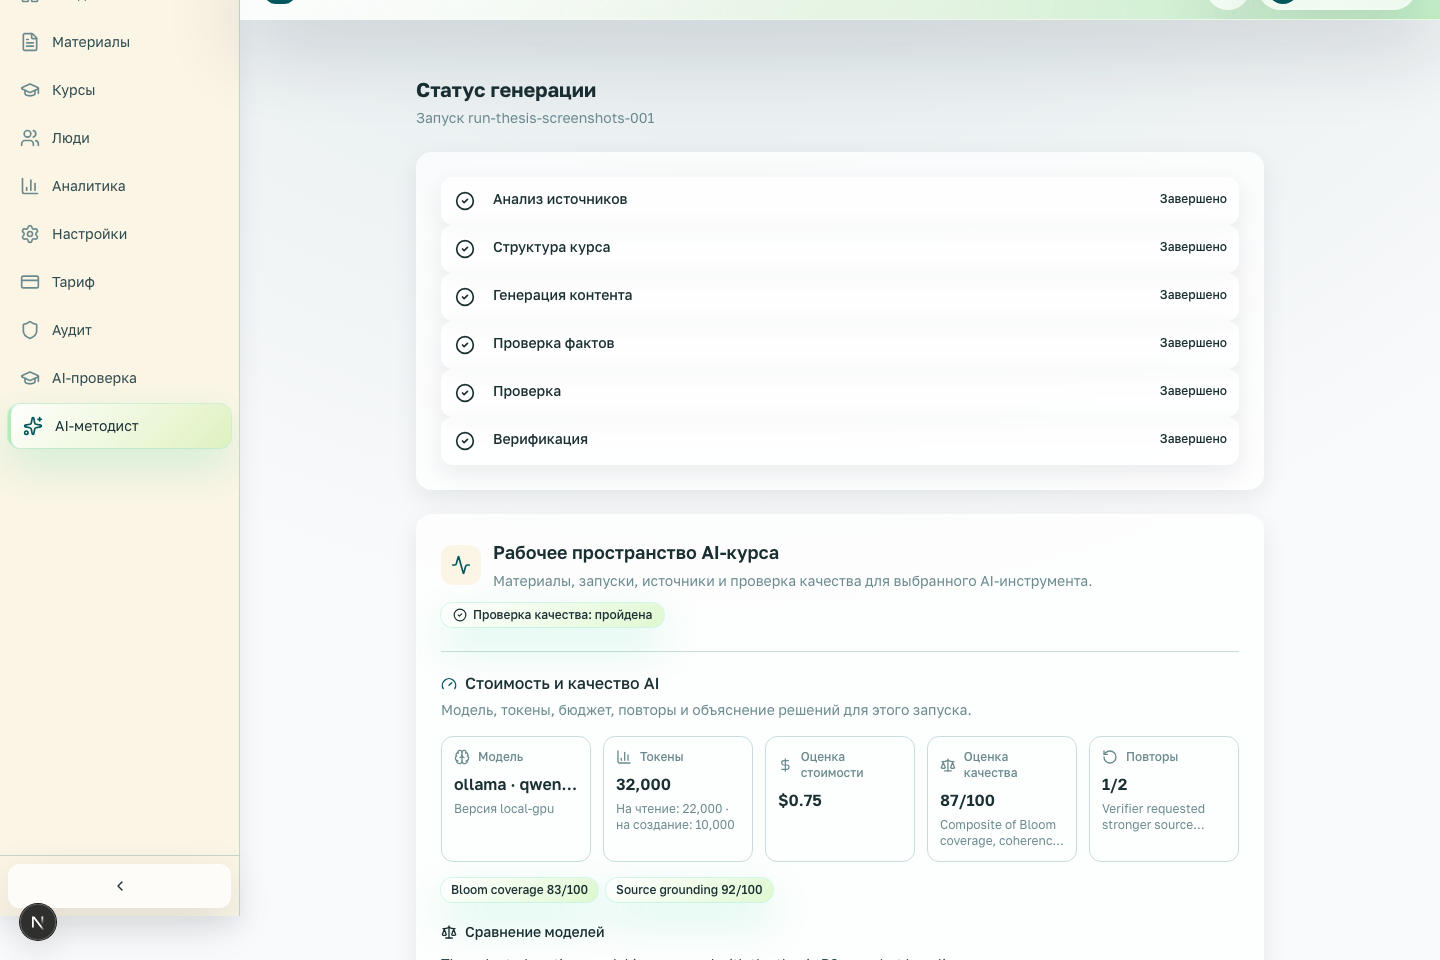
\includegraphics[width=0.98\textwidth]{figures/ui/ai-methodist-02-status.png}
  \caption{Экран статуса генерации, стоимости и качества запуска AI-методиста}
  \label{fig:ai-methodist-status}
\end{figure}

\section*{Л.3 --- Метрики дипломной валидации}

На~рисунке~\ref{fig:ai-methodist-thesis-validation} показан блок
дипломной валидации. Он фиксирует выполнение критериев H1--H3,
включая время до~первого черновика, Bloom coverage, source grounding
и~стоимость относительно ручной разработки. В~том~же интерфейсном
блоке показано paired-сравнение B1/B2/B3/B4 на~одном источнике.

\begin{figure}[p]
  \centering
  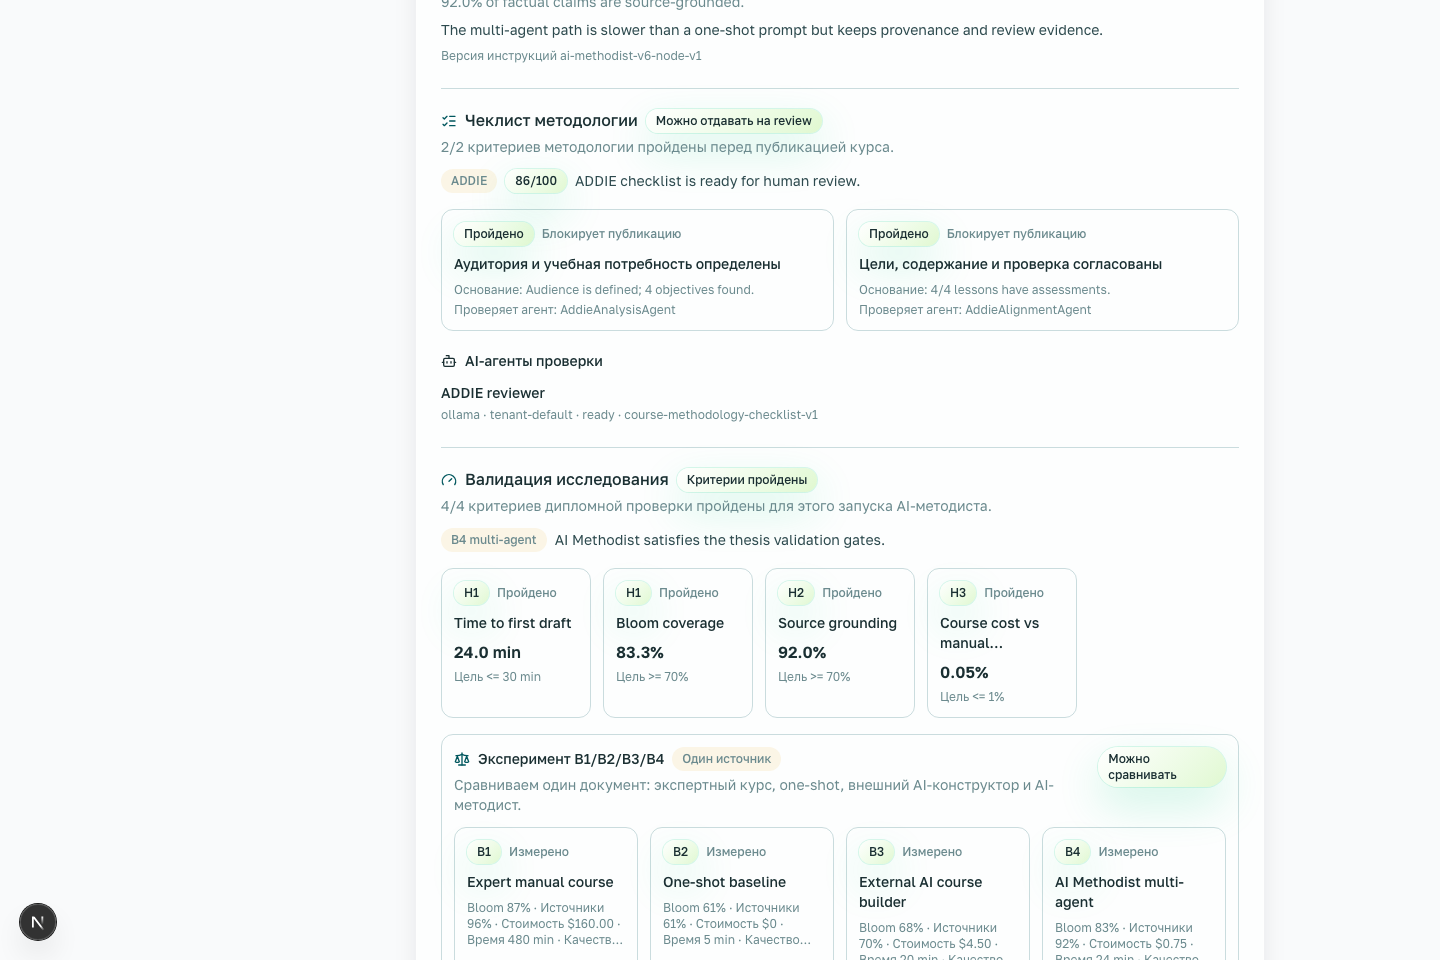
\includegraphics[width=0.98\textwidth]{figures/ui/ai-methodist-03-thesis-validation.png}
  \caption{Метрики дипломной проверки и paired-сравнение B1/B2/B3/B4}
  \label{fig:ai-methodist-thesis-validation}
\end{figure}

\section*{Л.4 --- Quality seal и источники}

На~рисунке~\ref{fig:ai-methodist-quality-seal} показаны загруженный
материал, история запуска, статусы генерации, источники и~итоговый
quality seal перед публикацией. Такой экран нужен комиссии как
подтверждение, что AI-методист не~ограничивается созданием текста:
результат сопровождается проверкой качества и~ссылками на~источники.

\begin{figure}[p]
  \centering
  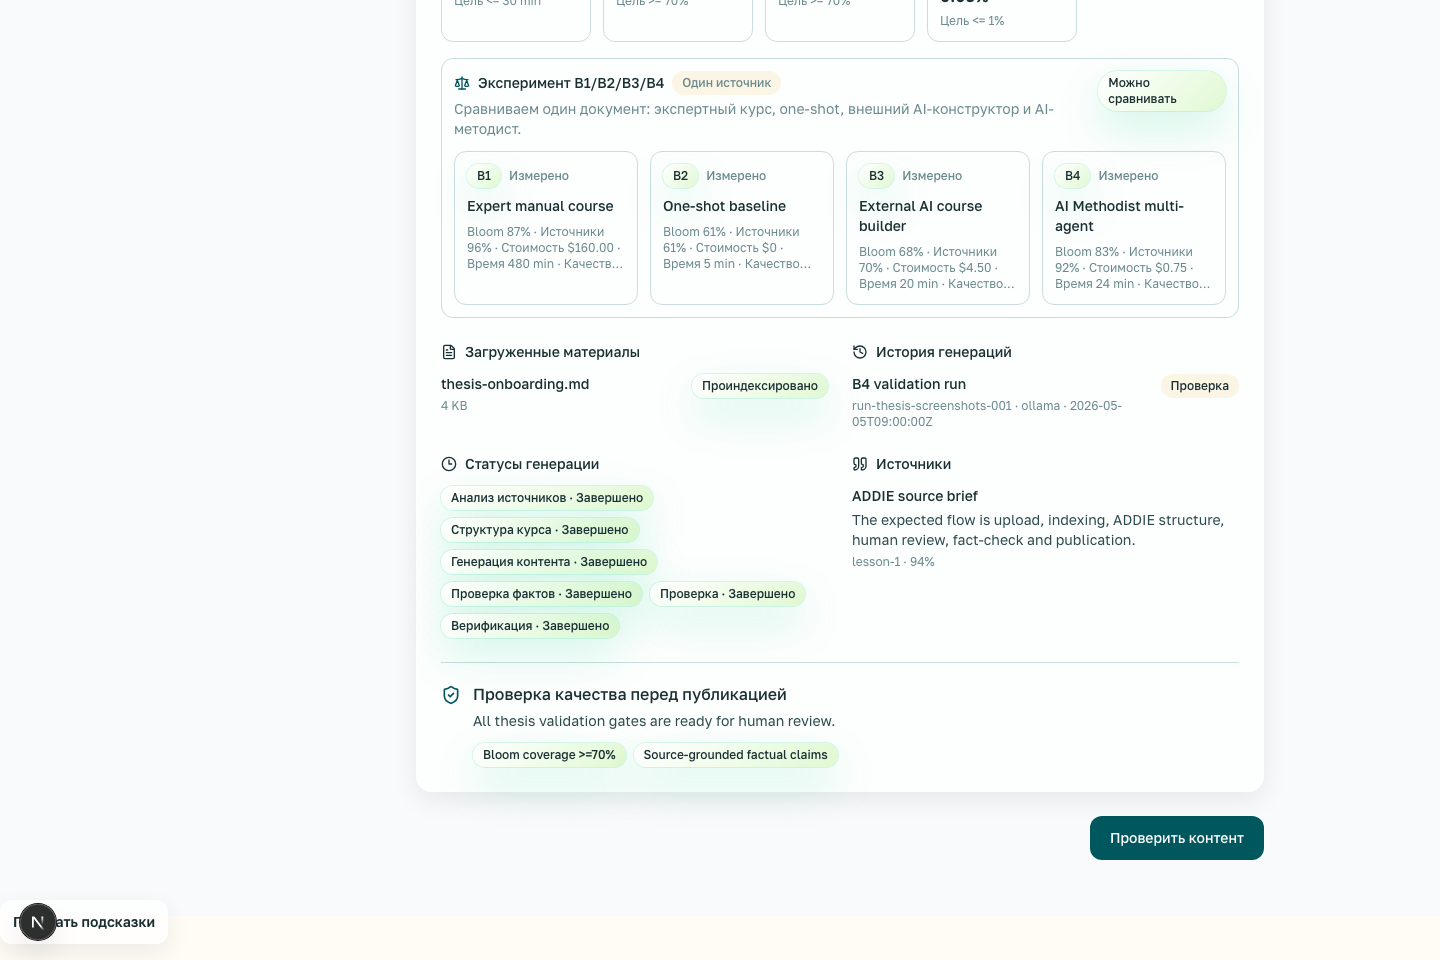
\includegraphics[width=0.98\textwidth]{figures/ui/ai-methodist-04-quality-seal.png}
  \caption{Quality seal, источники и история запуска AI-методиста}
  \label{fig:ai-methodist-quality-seal}
\end{figure}

\section*{Л.5 --- Provenance блоков курса}

На~рисунке~\ref{fig:ai-methodist-block-provenance} показан экран
проверки контента перед публикацией. Для каждого блока курса платформа
отображает источник, страницу, фрагмент, идентификатор запуска и~уровень
уверенности. Если источник отсутствует, интерфейс явно показывает
предупреждение, что блок нельзя считать полностью подтверждённым.

\begin{figure}[p]
  \centering
  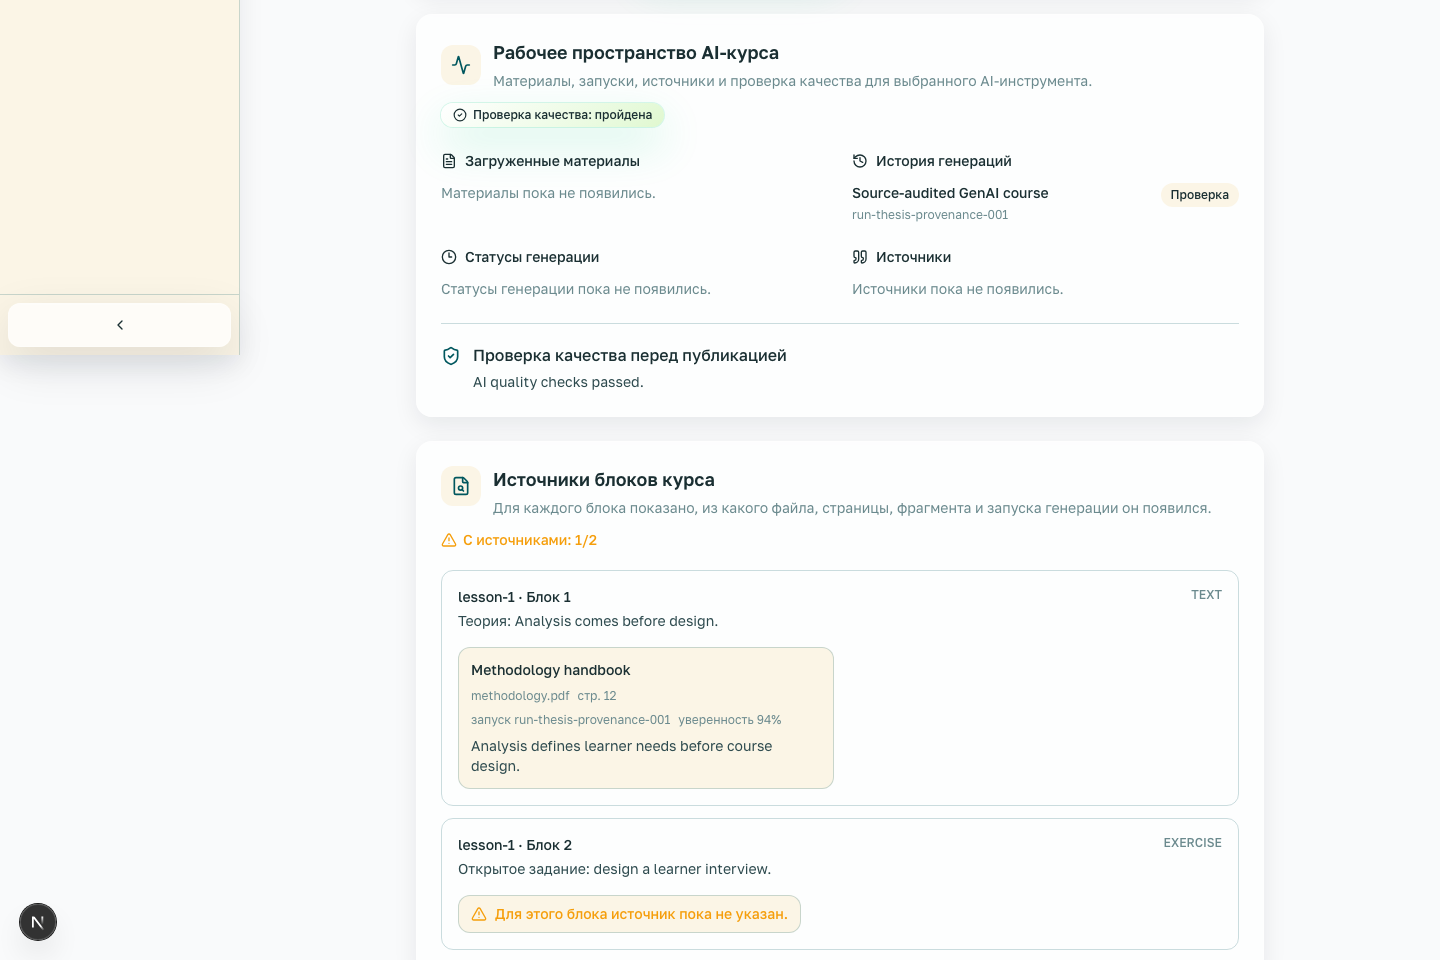
\includegraphics[width=0.98\textwidth]{figures/ui/ai-methodist-06-block-provenance.png}
  \caption{Block-level provenance: источник, страница, фрагмент и предупреждение о неподтверждённом блоке}
  \label{fig:ai-methodist-block-provenance}
\end{figure}
